\documentclass[11pt,a4paper]{article}
\usepackage[T1]{fontenc}
\usepackage{graphicx}
\usepackage[utf8]{inputenc}
\usepackage[margin=23mm]{geometry}
\usepackage{parskip}
\usepackage{amsmath}
\usepackage{longtable,array}
\usepackage{xcolor}
\usepackage{listings}
\usepackage{tikz}
\usetikzlibrary{arrows.meta,positioning}
\usepackage[hidelinks]{hyperref}
\lstset{basicstyle=\ttfamily\small,breaklines=true,columns=fullflexible,keepspaces=true,frame=single}
\tikzset{box/.style={draw,rounded corners,align=center,text width=65mm,minimum height=9mm,font=\small},arr/.style={-{Stealth},thick}}
\title{PointPillars Project: Filtering, Deployment, RViz and LiDAR Timestamps\\Complete Discussion Record}
\author{MasterThesis project}
\date{23 October 2026}

% Locate illustration assets from docs/ or the repository root. The built-in
% standalone compiler may not receive other project files; warn visibly then.
\newcommand{\projectshot}[2]{%
  \IfFileExists{figures/#1}{\includegraphics[width=#2]{figures/#1}}{%
    \IfFileExists{docs/figures/#1}{\includegraphics[width=#2]{docs/figures/#1}}{%
      \PackageWarningNoLine{project}{Screenshot #1 unavailable; illustrated output incomplete}%
      \fbox{\parbox{.85\linewidth}{\centering\small Screenshot asset unavailable.\par
      Keep \texttt{\detokenize{#1}} in the project's figures folder.\par
      See docs/figures/README.md for the original image and provenance.}}}}}

\begin{document}
\maketitle
The original discussion was recorded on 13 October 2026. A dated results continuation was added on 23 October; it is a documentation summary, not a verbatim extension of the transcript. The original record follows.

This standalone document records every substantive question, explanation, command, code excerpt, qualification and figure in the current chat up to the request to create this document. Chat interface metadata and raw tool output are not part of the discussion transcript. Diagrams originally written as Mermaid or text are reproduced below as editable TikZ figures or verbatim diagrams. The explanations describe the repository state inspected during the chat; they do not claim new runtime tests.
\tableofcontents
\newpage

\section{How the filtering algorithm currently works and what to do next}
\textbf{User:} ``How the filtering algorithm currently work and what is the suggested to do in the current state''

\textbf{Inspection update:} The project filtering code and notes were checked to explain the implementation and the suggested next steps.

The current filtering uses \textbf{Non-Maximum Suppression (NMS)} to remove overlapping detections. The recommendation is to investigate voxel capacity and the model's input conventions first, before tuning NMS.

The pipeline works as follows:
\begin{enumerate}
\item Validate the point cloud: reject malformed or oversized input, remove points containing NaN or infinite values, and divide intensity by \texttt{intensity\_scale}, whose default is 1.0.
\item Run the model. Its decoder has a confidence threshold of approximately 0.1.
\item Sort candidate boxes by confidence. Consider at most the highest-scoring 4096 candidates.
\item Keep the highest-scoring remaining box, then remove other boxes whose rotated bird's-eye-view IoU with it is at least 0.01. Repeat until all candidates are considered.
\item Publish the surviving boxes.
\end{enumerate}
The overlap calculation uses the boxes' rotated ground footprints. Height and vertical position do not affect suppression. Production filtering is class-agnostic: overlapping boxes can suppress each other even if their predicted classes differ.

For two ground footprints $A$ and $B$,
\[
\mathrm{IoU}(A,B)=\frac{\mathrm{area}(A\cap B)}{\mathrm{area}(A)+\mathrm{area}(B)-\mathrm{area}(A\cap B)}.
\]
The formula is explanatory notation for the overlap described in the chat. Implementation reference: \texttt{src/postprocess.cpp}, starting at line 120 in the inspected version.

\begin{center}
\begin{tabular}{p{.35\linewidth}p{.55\linewidth}}
\hline
Change & Expected effect\\\hline
Increase confidence threshold & Remove more low-confidence candidates.\\
Increase NMS IoU threshold & Keep more overlapping boxes, potentially including duplicates.\\\hline
\end{tabular}
\end{center}
Neither change guarantees better accuracy. NMS cannot correct misplaced boxes.

The evidence suggests this order of work:
\begin{enumerate}
\item \textbf{Verify bounded voxelization and repeatability.} Twelve of the 32 evaluated clouds exceeded the export's 10,000-voxel limit. Two diagnostic controls limiting inputs to 10,000 voxels and 32 points per voxel improved repeat matching to approximately 99.6--100\%. This supports investigating capacity and point selection; it does not yet prove an accuracy improvement.
\item \textbf{Establish the original training/input contract.} Check sensor height, coordinate conventions, intensity normalization, voxel features, and decoded box-center semantics. Matched cars showed approximately 1.53 m upward error, already present before ROS publication.
\item \textbf{Validate any justified correction on untouched data.} If accuracy remains poor after those checks, evaluate a model trained or fine-tuned for the intended sensor/domain.
\item \textbf{Then tune confidence, NMS IoU, and possibly class-aware suppression} using tuning data.
\end{enumerate}
Our NMS and NVIDIA's original NMS selected identical boxes across 192 saved observations. Filtering is therefore a lower-priority explanation for the broad accuracy failure. The recorded evaluation still had zero moderate-difficulty 3D matches on the small diagnostic split; the root cause is not fully established. Evidence: \texttt{docs/MODEL\_REFERENCE\_COMPARISON.md}.

\section{Project flow from zero to publication and RViz}
\textbf{User:} ``I would like to understand the project flow from 0 to pulish to riviz''

\textbf{Inspection update:} The startup, point-cloud input, inference, detection publication and RViz display paths were traced.

The project takes one LiDAR scan, runs the PointPillars model on the GPU, filters predicted boxes on the CPU, and publishes them through ROS 2. RViz subscribes to both the scan and the boxes to display them together. There are two parts: preparing the system once, then processing every incoming scan.

\begin{figure}[htbp]
\centering
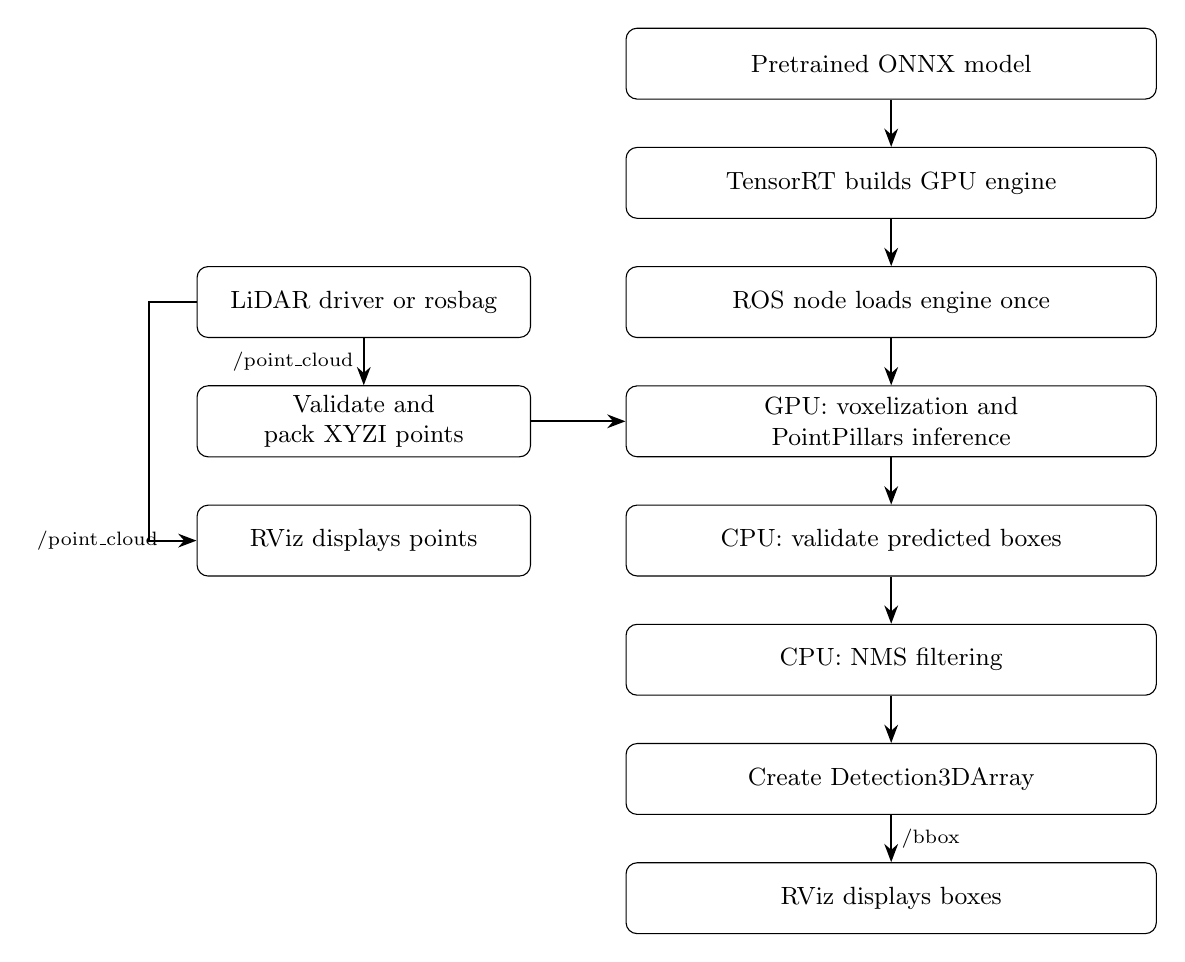
\begin{tikzpicture}[node distance=6mm]
\node[box] (onnx) {Pretrained ONNX model};
\node[box,below=of onnx] (engine) {TensorRT builds GPU engine};
\node[box,below=of engine] (load) {ROS node loads engine once};
\node[box,below=of load] (gpu) {GPU: voxelization and\\PointPillars inference};
\node[box,below=of gpu] (check) {CPU: validate predicted boxes};
\node[box,below=of check] (nms) {CPU: NMS filtering};
\node[box,below=of nms] (msg) {Create Detection3DArray};
\node[box,below=of msg] (rviz) {RViz displays boxes};
\node[box,text width=40mm,left=12mm of gpu] (pack) {Validate and pack XYZI points};
\node[box,text width=40mm,above=of pack] (source) {LiDAR driver or rosbag};
\node[box,text width=40mm,below=of pack] (points) {RViz displays points};
\draw[arr] (onnx)--(engine);\draw[arr] (engine)--(load);\draw[arr] (load)--(gpu);
\draw[arr] (source)--node[left,font=\scriptsize]{/point\_cloud}(pack);
\draw[arr] (pack)--(gpu);\draw[arr] (gpu)--(check);\draw[arr] (check)--(nms);
\draw[arr] (nms)--(msg);\draw[arr] (msg)--node[right,font=\scriptsize]{/bbox}(rviz);
\draw[arr] (source.west) -- ++(-6mm,0) |- node[pos=.7,left,font=\scriptsize]{/point\_cloud}(points.west);
\end{tikzpicture}
\caption{Complete project flow. This reproduces the Mermaid figure from the chat.}
\end{figure}

\subsection{Step 0: Prepare the computer}
The inference computer needs an NVIDIA GPU, a working NVIDIA driver, Docker, and NVIDIA Container Toolkit. The current deployment runs ROS 2 Jazzy, CUDA, TensorRT and the compiled project inside Docker. RViz runs separately on the desktop and needs host ROS Jazzy plus the \texttt{vision\_msgs} RViz plugin.

\subsection{Step 1: Build the application and obtain the model}
From the project directory:
\begin{lstlisting}
sudo bash tools/deploy.sh
\end{lstlisting}
Deployment builds the Docker image, obtains the published project source, downloads and verifies the pretrained ONNX model, and compiles the C++ ROS package. The ONNX file contains the trained network and its weights. This project performs inference; these steps do not train it again.

The normal Docker build obtains source from GitHub, so local unpushed changes are not included.

\subsection{Step 2: Convert ONNX into a TensorRT engine}
At container startup, the script checks whether a matching engine already exists. If it exists, startup reuses it. Otherwise, \texttt{trtexec} converts the ONNX model into an engine for the selected GPU and saves it in the persistent \texttt{pp-engines} volume. The current recipe builds an FP32, batch-one engine with TF32 disabled. Think of ONNX as the network description and the engine as its GPU execution version.

\subsection{Step 3: Start the ROS inference node}
The container starts the node as \texttt{/pointpillars}. It loads the engine once and creates the TensorRT execution context, CUDA stream and reusable GPU buffers. It then waits for point clouds.
\begin{center}
\begin{tabular}{lll}
\hline
Topic & Message type & Purpose\\\hline
\texttt{/point\_cloud} & \texttt{sensor\_msgs/msg/PointCloud2} & Incoming scans\\
\texttt{/bbox} & \texttt{vision\_msgs/msg/Detection3DArray} & Predicted boxes\\\hline
\end{tabular}
\end{center}
This connection is implemented in \texttt{src/pp\_inference\_node.cpp}.

\subsection{Step 4: A LiDAR driver or rosbag publishes a scan}
The detector needs a source of points: a live LiDAR driver or recorded bag playback. Each PointCloud2 message contains point data including x, y, z and intensity; a timestamp identifying when the scan was recorded; and a frame ID identifying its coordinate system, such as \texttt{velodyne}.

For the provided KITTI demo, start playback in another terminal:
\begin{lstlisting}
bash tools/rosbag_demo.sh
\end{lstlisting}

\subsection{Step 5: The CPU validates and prepares points}
For each incoming message, the callback checks the message layout, required fields, byte size and point capacity; converts the cloud into PCL XYZI points; removes points containing NaN or infinite values; divides intensity by the configured intensity scale; and packs remaining points into a continuous array:
\begin{lstlisting}
[x0, y0, z0, intensity0,
 x1, y1, z1, intensity1,
 ...]
\end{lstlisting}
Malformed input is dropped. A valid cloud with no remaining points produces an empty detection message. Implementation: \texttt{src/pointcloud\_adapter.cpp}.

\subsection{Step 6: The GPU executes PointPillars}
The application clears unused input padding, copies packed points and their count to the GPU, and executes the loaded engine. Conceptually:
\begin{lstlisting}
Points
  -> Group points into vertical pillars
  -> Extract features for each pillar
  -> Arrange features into a bird's-eye-view feature map
  -> Run the detection network
  -> Decode candidate object boxes
\end{lstlisting}
A candidate contains:
\begin{lstlisting}
x, y, z, length, width, height, yaw, class_id, score
\end{lstlisting}
The export class order is:
\begin{lstlisting}
0 = Vehicle
1 = Pedestrian
2 = Cyclist
\end{lstlisting}
These are intermediate predictions; filtering still follows. Implementation: \texttt{src/pointpillar.cpp}.

\subsection{Step 7: The CPU checks and filters candidate boxes}
The application copies results back from the GPU and validates output count, geometry, class IDs and scores. CPU NMS sorts boxes by descending confidence, considers up to 4096 candidates, keeps the highest-scoring remaining box, suppresses other boxes with rotated ground-footprint IoU at least 0.01, and repeats. The current production call uses class-agnostic suppression. NMS selects boxes; it does not move or resize them.

\subsection{Step 8: Create and publish the ROS detection message}
Surviving boxes become a Detection3DArray. For each box, the application writes center, dimensions, class ID and score, and converts yaw into a quaternion for orientation. It preserves the original scan's timestamp and frame ID, then publishes on \texttt{/bbox}. Preservation lets consumers associate detections with their source scan and interpret coordinates correctly. If inference fails, the frame is dropped and the node logs the error.

\subsection{Step 9: RViz receives and draws results}
With inference and the source running, open another terminal:
\begin{lstlisting}
bash tools/visualize.sh
\end{lstlisting}
The saved configuration subscribes to \texttt{/point\_cloud} to draw points and \texttt{/bbox} to draw predicted boxes using the vision\_msgs display plugin. Its fixed frame is \texttt{velodyne} for the tested KITTI bag. Another sensor frame requires a matching fixed frame or valid TF transform. RViz, inference and playback need the same \texttt{ROS\_DOMAIN\_ID}.

RViz performs visualization: the model and NMS have already finished before boxes reach it.

The ordinary startup sequence is:
\begin{lstlisting}
Terminal 1: sudo bash tools/deploy.sh
Terminal 2: bash tools/rosbag_demo.sh
Terminal 3: bash tools/visualize.sh
\end{lstlisting}
The complete message flow has been verified with actual bag playback and RViz rendering. Detection accuracy remains unresolved. The current node processes inference directly in its callback with queue depth 700. A bounded latest-frame worker is still pending, so overloaded processing can accumulate delayed scans.

\section{How direct RViz display was solved}
\textbf{User:} ``In the past this project wasn't able to display directly to riviz how you solved this ?''

\textbf{Inspection update:} Migration notes were checked to identify the changes that enabled direct display.

The project already published detection messages, but RViz needed a plugin to understand them, a configured view and working communication with Docker. These parts were solved together.
\begin{enumerate}
\item \textbf{Added the detection display plugin.} The node publishes \texttt{/bbox} as Detection3DArray. Host RViz was installed, but \texttt{vision\_msgs\_rviz\_plugins} was missing. Adding the official plugin allowed RViz to draw messages directly as 3D boxes.
\item \textbf{Added a saved RViz configuration.} \texttt{rviz/pointpillars.rviz} configures a point-cloud display on \texttt{/point\_cloud}, a detection display on \texttt{/bbox}, reliable QoS for both displays, fixed frame \texttt{velodyne} matching tested KITTI data, and colors for the three numeric class IDs.
\item \textbf{Fixed Docker-to-desktop communication.} Initially the host subscriber did not receive container messages through Fast DDS's default shared-memory transport. The root container and desktop user had an ownership-related transport problem. Using the following allowed messages to reach the host:
\begin{lstlisting}
export FASTDDS_BUILTIN_TRANSPORTS=UDPv4
\end{lstlisting}
The viewer launcher now applies this default and uses the selected ROS domain ID.
\item \textbf{Updated message construction for ROS Jazzy.} Migration updated class/score fields to the current vision\_msgs schema, preserved scan timestamp and frame ID, and populated box orientation and hypothesis pose.
\item \textbf{Wrapped setup in one launcher.} \texttt{tools/visualize.sh} finds the plugin, or prepares a local copy when possible, sets the transport environment and opens the saved view:
\begin{lstlisting}
bash tools/visualize.sh
\end{lstlisting}
\end{enumerate}
The resulting connection is:
\begin{lstlisting}
Inference node -> /bbox (Detection3DArray)
               -> RViz detection plugin -> visible 3D boxes

LiDAR / rosbag -> /point_cloud
               -> RViz point-cloud display -> visible points
\end{lstlisting}
No MarkerArray conversion was added: the plugin reads detection messages directly. Actual bag playback verified host message reception and live rendering of points and boxes. Inference and playback must already be running; visualize.sh starts only the viewer.

\section{Where the plugin integration is in the code}
\textbf{User annotation:} Selected ``Adding the official plugin allowed RViz to draw these messages directly as 3D boxes.'' Asked: ``in which part of the code you did this''

This was added in the RViz launcher and configuration, rather than the inference code:
\begin{itemize}
\item \texttt{tools/visualize.sh}, line 22 in the inspected version, checks whether vision\_msgs\_rviz\_plugins is installed. If missing, it downloads and extracts the official package locally, then adds its paths to \texttt{AMENT\_PREFIX\_PATH} and \texttt{LD\_LIBRARY\_PATH} so RViz can discover and load it.
\item \texttt{rviz/pointpillars.rviz} activates the plugin and connects it to published detections:
\end{itemize}
\begin{lstlisting}
- Class: vision_msgs_rviz_plugins/Detection3DArray
  Name: Detections
  Enabled: true
  Topic:
    Value: /bbox
\end{lstlisting}
The plugin's drawing implementation comes from the official ROS package. Our code makes that plugin available and configures it to read \texttt{/bbox}.

\section{LiDAR timestamps and how scanning starts}
\textbf{User annotation:} Selected ``A timestamp identifying when the scan was recorded.''

\textbf{User:} ``I would like to uderstand this , How the lidar works with this timestamp ? how i make the lidar start it's scan''

The timestamp is a time label attached to a scan. It tells software when measurements were acquired; it does not tell the LiDAR to start scanning.

The usual sequence is:
\begin{lstlisting}
LiDAR measures distances
    -> Driver collects measurements into a point cloud
    -> Driver attaches a timestamp and coordinate frame
    -> Driver publishes the cloud
    -> Our detector processes it
\end{lstlisting}
A LiDAR emits laser pulses and measures their returns to estimate distances. Depending on the sensor, it rotates or steers its beams to measure different directions. A cloud contains many measurements collected over a short interval, rather than all at exactly one instant.

In ROS 2 the cloud has a header such as:
\begin{lstlisting}
header:
  stamp:
    sec: 123
    nanosec: 500000000
  frame_id: velodyne
\end{lstlisting}
Here stamp represents 123.5 seconds on the clock used by the publisher. Depending on the driver, it may represent the beginning or end of the scan, or another acquisition reference. Some drivers also provide individual point timestamps.

Our project reads that header and copies it to the detection message. For example:
\begin{lstlisting}
Scan acquired:       10:00:00.100
Processing finishes: 10:00:00.150
Detection timestamp: 10:00:00.100
\end{lstlisting}
This means ``these boxes belong to the scan acquired at .100.'' Preserving acquisition time helps other software align detections with camera images, vehicle motion and coordinate transforms.

To start a real LiDAR, generally:
\begin{enumerate}
\item Power it and connect its network or USB interface.
\item Configure the connection and sensor settings.
\item Start its manufacturer-compatible ROS driver.
\item Enable scanning if that sensor requires a separate command.
\item Publish or remap the driver's point-cloud topic to \texttt{/point\_cloud}.
\end{enumerate}
The exact startup command depends on the LiDAR model. This project does not control LiDAR hardware; it subscribes to clouds supplied by its driver.

For the recorded KITTI demo, this supplies scans:
\begin{lstlisting}
bash tools/rosbag_demo.sh
\end{lstlisting}
It plays previously recorded clouds with recorded timestamps; it does not activate a physical sensor.

\textbf{Follow-up question asked in the chat:} ``Which LiDAR model are you using, or are you currently working only with the KITTI bag?'' No sensor model was provided before the document request, so a hardware-specific startup command remains unspecified.

\section{Document request and repository references}
\textbf{User:} ``Create a latex code contain everything in this chat even the figures , don't miss anything''

\textbf{Preparation update:} A standalone LaTeX document was requested containing all explanations, commands, code excerpts, follow-up questions and diagrams, to be opened in the built-in editor and checked for compilation.

All repository file references in the discussion are relative to:
\begin{lstlisting}
/media/ae/New Volume/MasterThesis
\end{lstlisting}
\begin{itemize}
\item \texttt{src/postprocess.cpp}: CPU rotated overlap and NMS.
\item \texttt{src/pp\_inference\_node.cpp}: subscription, callback and publication.
\item \texttt{src/pointcloud\_adapter.cpp}: XYZI preparation and ROS detection construction.
\item \texttt{src/pointpillar.cpp}: TensorRT engine loading and GPU inference.
\item \texttt{tools/deploy.sh}: deployment entry point.
\item \texttt{tools/rosbag\_demo.sh}: recorded KITTI input.
\item \texttt{tools/visualize.sh}: RViz launcher and optional plugin preparation.
\item \texttt{rviz/pointpillars.rviz}: saved point-cloud and detection display configuration.
\item \texttt{docs/MODEL\_REFERENCE\_COMPARISON.md}: independent comparison evidence and limitations.
\end{itemize}

\clearpage
\section{Results continuation: reviewed 23 October 2026}
The current local source baseline is \texttt{ee6b36c}. Numerical results retain
their original 3--14 October dates; the supplied screencast filenames are dated
20 October. This continuation updates project status without changing the
original questions and answers above.
\begin{longtable}{p{.29\linewidth}p{.62\linewidth}}
\hline Evidence & Result and interpretation \\ \hline
Labeled KITTI, 16 test frames, moderate &
Zero 3D matches for Car, Pedestrian and Cyclist. BEV AP R40 is
5.7516\%, 0\% and 0.02577\%. Vehicle is mapped to Car compatibility.
The 12 BEV-matched cars have median upward center error 1.529 m. \\
Independent reference &
TRT8 also reproduces poor accuracy/elevated centers. NVIDIA and project NMS
select identical boxes on 192/192 identical-candidate observations;
exact inference/training parity is still unaccepted. \\
Voxel-capacity controls &
12/32 original clouds exceed 10,000 pillars. Two tuning-only capped-input
controls improve repeat matching to about 99.6--100\%, without an accuracy
claim or installed production change. \\
Ouster feature experiment &
Raw signal rejects 15/48 observations with 33 nonfinite-length rows.
The three normalized encodings reject 0/144 observations. Only the fourth
feature changes. Accuracy/training calibration are not established. \\
Complete normalized Ouster replay &
Reflectivity/255 matches all 291+265 input/output occurrences without recorded
detector errors. Source duplicate headers are counted as occurrences. \\
Ouster camera and original-data view &
111 images, 111 CameraInfo messages and 556 normalized clouds are preserved.
Five raw/normalized cloud pairs pass non-intensity byte comparisons.
Camera/LiDAR header clocks remain different; no calibrated image overlay. \\
Frontal KITTI raw drive 0005 &
154 matched clouds/detections/images/CameraInfo messages; original XYZI and camera
pixels preserved. Full scans contain 98,532--124,122 points; no front-only crop.
This is an integration clip, not the labeled accuracy set. \\
\hline
\end{longtable}

\subsection{What the later sensor results change}
Unscaled Ouster signal is now a demonstrated contributor to numerical failures
on those recordings. Normalized features reduce excessive saturated predictions,
but do not resolve KITTI's vertical error or certify object correctness.
The ordinary Ouster helper still defaults to raw signal; select the diagnostic
encoding explicitly. Keep detector intensity scale 1.0 for already converted inputs.
\begin{lstlisting}
PP_OUSTER_FEATURE=reflectivity_div255 bash tools/rosbag_ouster.sh
# Separate viewer terminal:
RVIZ_CONFIG="$PWD/rviz/ouster.rviz" bash tools/visualize.sh
# Alternative player for original geometry plus normalized input and camera:
bash tools/rosbag_ouster_detail.sh
# Alternative frontal KITTI player:
bash tools/rosbag_kitti_front.sh
\end{lstlisting}
Select one player at a time, after stopping conflicting playback, and use the
corresponding saved RViz profile and matching domain. These alternatives do not
start inference. Camera playback coordinates bag-record arrival times; retaining
headers does not prove sensor-clock synchronization. The detector still has no
hardware scan-start control, configurable sensor QoS or bounded worker.

\subsection{Figures extracted from the user's videos}
The local sources are the two WebM files in
\path{/media/ae/New Volume/datasets/vedios}, with filenames
\texttt{Screencast from 2026-10-20 14-09-09.webm} and
\texttt{Screencast from 2026-10-20 14-13-14.webm}.
\begin{figure}[htbp]
\centering\projectshot{rviz-screencast-1.png}{.93\linewidth}
\caption{First recording, 32.035 s. RViz displays points, candidate boxes and
scores. No reviewed ground truth is shown.}
\end{figure}
\begin{figure}[htbp]
\centering\projectshot{rviz-screencast-2.png}{.93\linewidth}
\caption{Second recording, 16.023 s. Wider scene detail. Bag, engine and feature
identity cannot be established from the screenshot alone.}
\end{figure}
Full frames are retained losslessly without crop, resize or annotation.
\path{docs/figures/provenance.json} records source/image hashes and timestamps.
The figures demonstrate visible rendering in the supplied recordings; they do
not demonstrate detection accuracy, latency or calibrated camera projection.

\subsection{Verification, attribution and next work}
The documentation review passed 64 existing Python tests and rehashed the selected
saved result JSON evidence against inventories. No new GPU run, model adaptation,
threshold tuning or image rebuild was performed. Two earlier allocation memchecks
reported zero errors but do not complete internal tensor-bounds/race validation.
The runtime remains synchronous with reliable depth 700; worker/QoS/metrics,
original-training parity, larger untouched accuracy evaluation and CI remain open.

Ouster source attribution: Kenji Koide, AIST, DOI
\texttt{10.5281/zenodo.7780490}, CC-BY-4.0. KITTI attribution: Geiger, Lenz,
Stiller and Urtasun, KIT/TTI-C, CC-BY-NC-SA-3.0. Screenshot experiment identity
is not independently established. Preserve the relevant source terms with data.
See \path{docs/CURRENT_STATUS_AND_RESULTS.md} for the consolidated tables and
\path{recovery/PROGRESS.md} for final link/asset/compiler verification.

\end{document}
